\begin{frame}{Implementação}
    \begin{itemize}
        \item Foi implementado uma formalização de caminhos ponderados
        \begin{itemize}
            \item [--] Os pesos foram restritos aos números naturais
            \item [--] Os códigos estão disponíveis em \url{https://github.com/joao-frohlich/dijkstra-coq}
        \end{itemize}
        \item As seguintes propriedades foram provadas
        \begin{enumerate}
            \item Todo caminho é positivo
            \item A adição de um vértice ao início de um caminho qualquer $C$ faz com que o peso deste novo caminho seja igual ao peso de
            $C$ somado ao peso definido para a aresta que liga este novo vértice ao primeiro vértice de $C$;
            \item O peso da concatenação de dois caminhos $C_1$ e $C_2$, desde que obedecendo às restrições impostas pela função de
            concatenação de caminhos, será igual à soma do peso de $C_1$ com o peso de $C_2$.
        \end{enumerate}
    \end{itemize}
    % \begin{figure}[htbp]
    %     \centering
    %     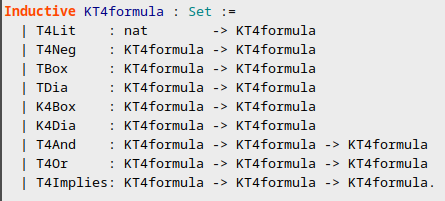
\includegraphics[scale=.6]{LinguagemKT4.png}
    %     \caption{Linguagem de \(\textbf{KT} \odot \textbf{K4}\)}
    % \end{figure}
\end{frame}